\documentclass[11pt]{article}

\usepackage{fullpage}
\usepackage{mathptmx}
\usepackage{latexsym}
\usepackage{graphicx}
\usepackage{amsmath, amssymb, amsthm, amsfonts}
\usepackage{algpseudocode}

\newcommand{\handout}[5]{
   \renewcommand{\thepage}{#1-\arabic{page}}
   \noindent
   \begin{center}
   \framebox{
      \vbox{
    \hbox to 5.78in { {\bf COMPSCI 634: Geometric Algorithms} \hfill #2 }
       \vspace{4mm}
       \hbox to 5.78in { {\Large \hfill #5  \hfill} }
       \vspace{2mm}
       \hbox to 5.78in { {\it #3 \hfill #4} }
      }
   }
   \end{center}
   \vspace*{4mm}
}

\renewcommand{\paragraph}[1]{\medskip \noindent {\bf #1.}}

\newcommand{\lecture}[4]{\handout{#1}{#2}{Lecturer: #3}{Scribe: #4}{Lecture #1}}

\newtheorem{definition}{Definition}
\newtheorem{algorithm}{Algorithm}
\newtheorem{openquestion}{Open Question}
\newtheorem{remark}{Remark}
\newtheorem{theorem}{Theorem}
\newtheorem{lemma}[theorem]{Lemma}
\newtheorem{corollary}[theorem]{Corollary}
\newtheorem{fact}[theorem]{Fact}

\newcommand{\example}[1]{\paragraph{Example #1}}

\begin{document}

\lecture{\#24: Geometric Set Cover}{4/3/2014}{Pankaj Agarwal}{Chris Tralie}	



\section{Overview}
\label{section:overview}

The purpose of this lecture is to cover a few classic combinatorial optimization problems, including set cover, hitting set, and independent set, in a geometric context.  Though the optimal set cover and hitting set problems are NP-hard, results from $\epsilon$-nets help to give good approximation bounds for these algorithms for simpler set systems that arise in a geometric context.

The notes begin with some preliminary definitions of the dual range space and of the algorithms, and several results from $\epsilon$-nets are reviewed.  Then, a modified, weighted version of an $\epsilon$-net is presented which leads to an approximation algorithm for the hitting set and set cover.  After this, a new randomized hitting set algorithm with better bounds is presented, which was discovered by our very own T.A. Jiangwei Pan and professor Pankaj Agarwal.  Finally, some basic ideas for independent set are shown in a geometric context

Throughout, I also highlight several open problems that were mentioned in class.

\section{Dual Range Spaces}
\label{section:dualrangespaces}

\subsection{Definitions}

\begin{definition}

Let $\Sigma = (X, R)$ be a range space on the set $X$.  Then

\[ \Sigma^T = \left( R, \{ \{ r_j | x_i \in r_j \} | x_i \in X \} \right) \]

is the {\em dual range space} associated with $\Sigma$

\end{definition}

In other words, the space becomes the set of ranges, and the ranges become sets of ranges that hit an $x \in X$.  A slightly easier conceptualization of a range space for this purpose is a bipartite graph, where one set is the elements in $X$ and the other set is the ranges, and there's a line between $x \in X$ and $r \in R$ if $x \in r$.  The dual range space simply switches the roles of the two sets in the graph.  Figure~\ref{fig:BipartiteGraph} shows an example with this construction.

\begin{figure}[h]
\centering
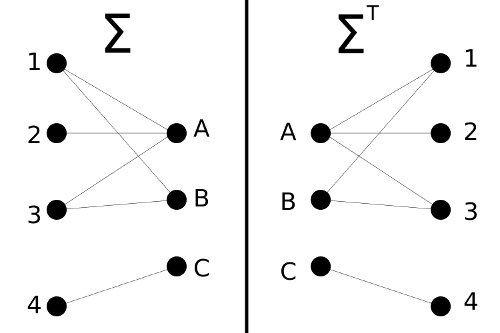
\includegraphics[width=0.4\textwidth]{BipartiteGraph.png}
\caption{An example of a range space represented as a bipartite graph.  The primal range space has $X = \{ 1, 2, 3, 4 \} , R = \{ \{1, 2, 3\}, \{1, 3\} \{ 4 \} \}$.  The dual range space has $X = \{A, B, C\}, R = \{ \{ A, B \}, \{ A \}, \{ A, B \}, \{ C \} \}$}
\label{fig:BipartiteGraph}
\end{figure}

Note also that if one constructs an incidence matrix $A$ for the range space out of this bipartite graph, then $A^T$ represents an incidence matrix for the dual range space.  This makes the transpose symbol a natural choice for denoting the dual range space.

\subsection{Geometric Example}
\label{sec:GeometricExample}

One way to visualize dual range spaces in a geometric context is with points and rectangles.  Define the following objects:

\begin{itemize}

\item $X$: Finite set of points in $\mathbb{R}^2$

\item $\gamma$: A finite set of $m$ rectangles $(\gamma_1, ..., \gamma_m)$

\item $\Sigma: (X, \{ \gamma \cap X | \gamma \in \Gamma \} ) $

In other words, for each rectangle, create a range comprised of the points that are contained within that rectangle

\item $\Sigma^T: ( \Gamma, \{ \{ \gamma | x \in \gamma\} | x \in X \} )$

In other words, for each point, create a range out of the set of rectangles that contain it

Figure~\ref{fig:RectanglePoints} shows an example of such a space.

\end{itemize}


\begin{figure}[h]
\centering
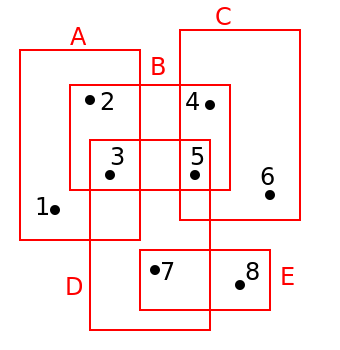
\includegraphics[width=0.5\textwidth]{RectanglePoints.png}
\caption{An geometric example of a range space.  The primal range space consists of the points $X = \{ 1, 2, 3, 4, 5, 6, 7, 8 \}$ and the rectangles covering the ranges  $R = \{ A:\{1, 2, 3\}, B:\{2, 3, 4, 5\}, C:\{4, 5, 6\}, D:\{3, 5, 7\}, E:\{7, 8\} \}$.  The dual range space consists of the rectangles $X = \{ A, B, C, D, E \}$ and the points intersecting the rectangles $R = \{ 1:\{A\}, 2:\{A, B\}, 3:\{A, B, D\}, 4:\{B, C\}, 5:\{B, C, D\}, 6:\{C\}, 7:\{D, E\}, 8:\{E\} \}$ }
\label{fig:RectanglePoints}
\end{figure}

\section{Geometric Hitting Set and Set Cover}
\subsection{Definitions}

\begin{definition}

For the range space $\Sigma = (X, R)$, $H \subset X$ is a {\em hitting set of $\Sigma$} if 

\[ H \cap r \neq \emptyset \forall r \in R \]

\end{definition}


\begin{definition}

For the range space $\Sigma = (X, R)$, $S \subset R$ is a {\em set cover of $\Sigma$} if
\[ \cup_{s \in S} s = X \]

\end{definition}

Note that the hitting set of a range space $\Sigma$ is the same as a set cover of $\Sigma^T$.  The goal is to find the smallest sized hitting set or set cover.  Note also that the hitting set is closely related to an $\epsilon-\text{net}$.  To see this, recall the definition of an $\epsilon-\text{net}$

\begin{definition}

$N \subset X$ is an {\em $\epsilon - \text{net}$} of $X$ if $\forall r \in R$ 

\[ |r| \geq \epsilon |x| \implies N \cap r \neq \emptyset \]

\end{definition}

If $\epsilon = \frac{1}{N}$ in the definition of the the $\epsilon$-net, where $N = |X|$ for the ranges space $\Sigma = (X, R)$, then the $\epsilon$-net is certainly a hitting set for all of the ranges, because every range has size at least 1.  Though the $\epsilon$ is quite small in this case, and it is only related to $N$, not to the optimal sized hitting set.  Still, if one can improve the bound on $\epsilon$, $\epsilon$-nets may be useful for set systems of bounded VC-dimension because of the following theorem

\begin{theorem}
\label{theorem:epsnettheorem}
	Given a range space $\Sigma = (X, R)$ with finite VC-dimension $d$, for any $\delta, \epsilon > 0$, a random subset $N \subset X$ of size 
	
\[ O\left( \frac{d}{\epsilon} \log \frac{1}{\delta \epsilon} \right) \]
 is an $\epsilon$-net of $\Sigma$ with probability $\geq (1 - \delta)$
 \cite{har2011geometric}
\end{theorem}

Thus, the hope is to come up with better approximation algorithms for simple set systems using this theorem.  As an example of where this may be useful, return to the ranges space with points and rectangles in Section~\ref{sec:GeometricExample}.  In fact, for this range space, an even better bound of size $O(\frac{1}{\epsilon} \log \log \frac{1}{\epsilon} )$ has been shown recently in \cite{aronov2010small}, while the $\epsilon$-net of the dual range space is still $O(\frac{1}{\epsilon} \log \frac{1}{\epsilon} )$ with constant probability.

As a side note, this implies that there is actually a gap in the bounds for computing set cover and the hitting set if $\epsilon$-nets are used for the approximation.

\subsection{An Approximation Algorithm}

As mentioned before, the goal is to somehow reduce the hitting set to an $\epsilon$-net.  The main issue with the $\epsilon$-net is that it is only guaranteed to cover heavy (high cardinality) ranges, but the hitting set requires all ranges to be covered, so before $\epsilon$ had to be set to a very small value $\frac{1}{N}$.  To make this more convenient for the hitting set application, modify the definition of an $\epsilon$-net to include weights for each element, so that small sets can effectively be given larger weights:

\begin{definition}

For a range set $\Sigma = (X, R)$, define a map 

\[w: X \rightarrow \mathbb{Z}^+\]

And extend this maps to sets $S \in R$ so that

\[ w(S) = \sum_{x \in S} w(x) \]

Then $N \subset X$ is a {\em weighted $\epsilon$-net of $(\Sigma = (X, R), w)$} if $\forall r \in R$

\[ w(r) \geq \epsilon w(x) \implies r \cap N \neq \emptyset \]

Also say that $r$ is {\em $\epsilon$-light} if $w(r) < \epsilon w(x)$

\end{definition}

Use this modified definition to devise an algorithm that estimates the weights $w$ for a range space $(\Sigma = (X, R), w)$ that will lead to a good hitting set approximation with an $\epsilon$-net.  The algorithm is as follows:

\begin{algorithm}
\fbox{
{\em
\begin{minipage}{0.5\textwidth}

\begin{algorithmic}
\State ALGORITHM HittingSetApprox1$(\Sigma = (X, R) )$
\State Initially, $w(x) = 1 \forall x \in X$

\While{$\exists$ an $\epsilon$-light range}

	\State Choose an $\epsilon$-light range $r \in R$
	
	\State $w(x) \leftarrow 2 w(x) \forall x \in r$
	
\EndWhile

\State \Return $\epsilon$-net of $(\Sigma, w)$
\end{algorithmic}

\end{minipage}
}
}
\label{alg:estimateweights}
\end{algorithm}

The algorithm is very simple, but the analysis requires some tricks.  To analyze this algorithm, let $w_i(x)$ be $w(x)$ after $i$ iterations.  Find an upper bound and a lower bound for $w_i(x)$.  Also let $H^*$ be an optimal hitting set algorithm of size $k$.

\begin{itemize}

\item To find an upper bound, observe that at each iteration, the weights of an $\epsilon$-light range $r$ are doubled.  Since by definition $w_i(r) < \epsilon$, 

\[ w_{i+1}(X) = w_i(X) + w_i(r) \leq (1 + \epsilon) w_i(X) \]

Since all of the weights start off at 1, $w_0(X) = n$.  Thus, the upper bound is 

\[ w_{i}(X) \leq n(1+\epsilon)^i \]


\item 
To find a lower bound, examine what happens to $w(H^*)$ after each iteration.  Note that at each iteration, at least one element in $H^*$ is doubled in weight.  For the first $k$ iterations, the minimum happens if these changes are spread out, so that a different element is doubled each time.  Thus,

\[ w(H^*) \geq k + i \]

Let $f(i) = k + i$ (spread the changes out evenly), and let $g(i) = k2^{i/k}$.  Then $f(i) > g(i)$ over $[0, k]$, because $f(0) = g(0)$, $f(k) = g(k)$, $f'(0) > g'(0)$, and they are both convex functions.  Also, each group of $k$ iterations after the first $k$ (for $i > k$), it is also true that the minimum is achieved by spreading the elements out.  Therefore, the lower bound over all $i$ elements doubled in weight is

\[ w(H^*) \geq k 2^{i/k} \]

\end{itemize}

To get $k = |H^*|$ involved in the upper bound, let

\[ \epsilon = \frac{\ln \sqrt{2}}{k} \]

, a choice which will become clear in a moment.  Then

\[ w_i(X) \leq (1 + \epsilon)^i n = \left(1 + \frac{\ln \sqrt{2}}{k} \right)^i n \leq  \exp\left(  i \frac{\ln \sqrt{2}}{k} \right) n\]

Since $H^* \subset X$,

\[ w_i(H^*) \leq w_i(X) \leq \exp\left(  i \frac{\ln \sqrt{2}}{k} \right) n \]

Now combine the lower bound and the upper bound on $w_i(H^*)$

\[ k 2^{i/k} \leq n \exp \left( i \frac{\ln \sqrt{2}}{k} \right) \]

\[ \ln(k) + \ln(2) \frac{i}{k} \leq \ln(n) + \ln \sqrt{2} \frac{i}{k} \]

In this step it is clear how clever the choice of $\epsilon = \frac{\ln \sqrt{2}}{k}$ is (it allows us to subtract $ \ln \sqrt{2} \frac{i}{k}$ from both sides of the inequality while maintaining a nonzero factor of $\frac{i}{k}$ on the left side)


\[ \frac{i}{k} \ln(\sqrt{2}) \leq \ln \left( \frac{n}{k} \right) \]

\[ i = O\left( k \log \frac{n}{k} \right) \]

The analysis so far has assumed the size of the optimal hitting set $k = |H^*|$, is known, but that information is not actually available up front.  To estimate $k$, pick start with a small value of $k$ (say 1), and do an exponential binary search, doubling $k$ if the algorithm above doesn't converge in $(k/\sqrt{2}) \log\left(\frac{n}{k}\right)$ steps.

When the algorithm finally terminates, the $\epsilon$-net of the weighted range space $(\Sigma, w)$ is an $O\left( k \log \frac{n}{k} \right)$ of the optimal hitting set of the ranges.  In practice, to transform the weighted $\epsilon$-net to an unweighted $\epsilon$-net so that ordinary $\epsilon$-net algorithms can be run, simply replicate the elements in $(\Sigma, w)$ by their weights (this is why it was important that $w$ be positive integer weights).


\begin{openquestion}
It is known that for a range space over points with ranges of discs, the size of the $\epsilon$-net is $\Theta(\frac{1}{\epsilon})$, so this algorithm gives a constant-sized approximation of the optimal hitting set for that special case.  However, it is not known whether we can beat the above bound for the special case of points and rectangles

\end{openquestion}

\subsection{Jiangwei and Pankaj's Approximation Algorithm}

\begin{algorithm}
\fbox{
{\em
\begin{minipage}{0.8\textwidth}

\begin{algorithmic}
\State ALGORITHM HittingSetApprox2$(\Sigma = (X, R) )$

\State

For the range space $\Sigma = (X, R)$
\begin{flalign}
 &\text{Let} \mu = \frac{2}{\ln 2} k \ln |R|^2|X|&
\end{flalign}
\State Initially, $w(x) = 1 \forall x \in X$
\State Initially, $w(r) = 1 \forall r \in R$

\For{$i = 1$ to $\mu$}

	\State 
	\begin{itemize}
	\item Sample a random $\overline{x_i} \in X$ with the probability distribution $\text{Pr}(x) = w(x)/w(X)$ 
	
	\item Sample a random range $\overline{r_i} \in R$ with the probability distribution $\text{Pr}(r) = w(r)/w(R)$
	
	\end{itemize}
	
	\State $\forall r \text{ s.t. } x_i \in r, w(r) \leftarrow w(r)/2 $
	
	\State $\forall x \in r, w(x) = 2w(x)$
	
\EndFor
\end{algorithmic}

\end{minipage}
}
}
\label{alg:jiangweialg}
\end{algorithm}

Let $\Pi(x_i)$ be the number of indices $k \leq \mu$ where $\overline{x_k}  = x_i$.  Then a $1/(8k)$-net of the weighted range space $(\Sigma, \Pi)$, is an $O(1)$ approximation of the optimal hitting set. More details can be found in \cite{pan2014hittingset}, particularly in Section 4 of that paper.


\section{Geometric Independent Set}

The independent set problem asks for the largest set system such that each set is pairwise disjoint.  This problem appears to be harder than hitting set and set cover to approximation.  In particular, for some independent sets of size $n/2$, the best known polynomial approximation algorithm returns a set system within $\log^2 n$ size of the optimal.

\begin{figure}[h]
\centering
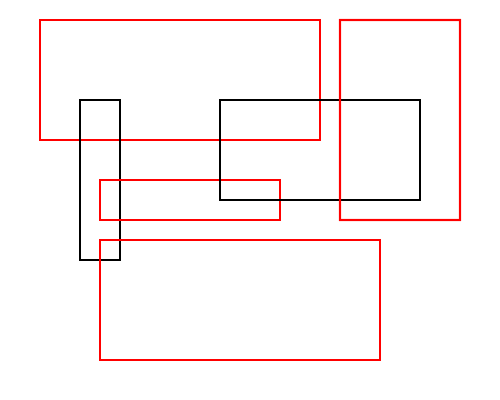
\includegraphics[width=0.5\textwidth]{RectangleIndySet.png}
\caption{A geometric example of an independent set.  The rectangles in the independent set are drawn with a red border}
\label{fig:RectangleIndySet}
\end{figure}

One geometric example is, given a set of axis-parallel rectangles $R$, find the largest subset $S \subset R$ such that $\forall r_1, r_2 \in S, r_1 \cap r_2 = \emptyset$.  An example is shown in Figure~\ref{fig:RectangleIndySet}.  An application of this example is to figure out how many city labels it is possible to display on a map without too much clutter (reduce to this problem by putting a bounding rectangle around each city label).

With the simpler example where all rectangles are unit-sized squares, a constant-factor approximation is possible with a simple greedy algorithm which takes a random square and removes the squares that intersect it, and repeats until there are no pairwise intersections.  To extend this to squares of different sizes, do the same, but choose the squares to check in increasing order of size.

For rectangles, a $\log n$ approximation is possible with the following greedy algorithm:

\begin{algorithm}
\fbox{
{\em
\begin{minipage}{0.8\textwidth}

\begin{algorithmic}
\State ALGORITHM 2DIS(R)

\State
Draw a vertical line $l$ s.t. each side contains an equal number of vertices on the rectangles $R$

\State Define the sets

\begin{itemize}

\item $R_0 = \{ r | l \cap r \neq \emptyset \}$
\item $R^- = \{ r | r \text{  lies to the left of } l \}$
\item $R^+ = \{ r | r \text{  lies to the left of } l \}$

\end{itemize}
	
\State Determine the independent set $I(R_0)$ with a 1D greedy algorithm.

\State Return $I(R) = I(R_0) \cup 2DIS(R^-) \cup 2DIS(R^+)$

\end{algorithmic}

\end{minipage}
}
}
\end{algorithm}

It is also possible to approximate this problem by formulating it as an integer linear programming and then rounding, but this is slower.

\begin{openquestion}
Is there a simple $O(\log\log n)$ factor approximation for the independent set of axis-aligned rectangle problem?
\end{openquestion}

\begin{openquestion}
Is there a simple $O(1)$ factor approximation for the independent set of axis-aligned rectangle problem?
\end{openquestion}


%Describe the problem crisply, followed by the results that we develop. If you feel the need to 
%further sub-divide the contents of this section to improve its organization, use subsections and
%paragraphs as shown below.

%\subsection{Subtopic}
%\label{subsection:subtopic}

%In this subsection, we give ....

%\begin{lemma}
%\label{lemma:somelemma}
%	Here goes the statement of the lemma.
%\end{lemma}
%\begin{proof}
%	Give a proof of the above lemma. Lemmas are technical statements
%	that are used in proving theorems. For an example, see below.
%\end{proof}

%\begin{theorem}
%\label{theorem:sometheorem}
%	Here goes the statement of the theorem.
%\end{theorem}
%\begin{proof}
%	Give a proof of the theorem (perhaps using Lemma~\ref{lemma:somelemma}).
%	Theorems are typically proved by using one or more lemmas, and represent
%	the final statement that you are trying to make in this topic. E.g., 
%	Algorithm A has a running time of $O(n^2)$ is a theorem, but Subroutine B
%	in Algorithm A has a running time of $O(n)$ is a lemma.
%\end{proof}

%\begin{corollary}
%\label{corollary:somecorollary}
%	Here goes the statement of the corollary.
%\end{corollary}
%\begin{proof}
%	Give a proof of the corollary (perhaps using Theorem~\ref{theorem:sometheorem}).
%	Corollaries are consequences of theorems.
%\end{proof}

%\begin{fact}
%\label{fact:somefact}
%	Here goes a fact. Facts are statements for which a proof was not furnished in lecture.
%	So you do not need to provide a proof either.
%\end{fact}

%\begin{definition}
%\label{definition:somedefinition}
%	Here goes a definition.
%\end{definition}

%\begin{remark}
%\label{remark:someremark}
%	Here goes a remark.
%\end{remark}

%\example{1} 
%\label{eg:someexample}
%Here is an example. Note that for examples, you can choose the numbering scheme. 
%In particular, use incremental numbering only if you are giving multiple examples 
%for the same thing. If you are giving only one example for anything, always call
%it Example 1.

%\paragraph{Mathematical formatting}
%You will be required to use a lot of mathematical formatting. A few examples:

%\begin{equation}
%\label{equation:someequation}
%	(a - b)^2 = a^2 - 2ab + b^2.
%\end{equation}

%\begin{eqnarray}
%	 (a-b)^2 & \geq & 0 \\
%	\Rightarrow \quad a^2 + b^2 & \geq & 2ab.
%\end{eqnarray}

%As far as possible, avoid inserting mathematical equations (or complicated expressions)
%inline.

%\section{TopicB}
%\label{section:topicb}

%(If several topics were covered in the lecture, use additional sections.) 
%In this section, we will describe a topic which is different from that in Section~\ref{section:topica}.

%\paragraph{References} You should be accurate with references. E.g., you may need to
%cite a book by Cormen {\em et al}~\cite{CormenLRS01} or a journal article by 
%Klein and Ravi~\cite{KleinR95} or a conference paper by Karger~\cite{Karger93}.
%Follow the convention given for bibtex entries in the scribe-notes-ref.bib file. The same file 
%should be used for all lectures. To avoid repeated entries, use lexicographical ordering
%on the names of the authors.

%\section{Summary}
%\label{section:summary}

%Give a short summary of the topics that we covered in this lecture. 

\bibliographystyle{alpha}
\bibliography{Notes_lec22-ref}

\end{document}
